


\begin{frame}
\frametitle{Take-Away Message}
\begin{itemize}
\item Visualization can help at different stages of \\the development process
\item Discover problems early
\item Understand what is happening without drowning in details
\item Easily communicate with stakeholders without CP experience 
\item Decide how much integration with solver you need
\item Complex use cases require visualization to be practical
\item Generic vs. application specific visualization 
\end{itemize}
\end{frame}

\begin{frame}{Lots of pretty pictures, too!}
\only<+->{\begin{textblock*}{6cm}(0cm,-3cm)
\includegraphics[width=4cm]{images/alldifferentexplanation}
\end{textblock*}}
\only<+->{\begin{textblock*}{6cm}(7cm,-3cm)
\includegraphics[width=8cm]{images/conflict-visualisations-mw}
\end{textblock*}}
\only<+->{\begin{textblock*}{6cm}(0cm,0cm)
\includegraphics[width=6cm]{images/oz_explorer_1.jpg}
\end{textblock*}}
\only<+->{\begin{textblock*}{6cm}(2cm,-1cm)
\includegraphics[width=11cm]{images/flowbound127pushed.PNG}
\end{textblock*}}
\only<+->{\begin{textblock*}{6cm}(3cm,0cm)
\includegraphics[width=8cm]{images/flowsearchcompare.PNG}
\end{textblock*}}
\only<+->{\begin{textblock*}{6cm}(6cm,-2cm)
\includegraphics[width=9cm]{images/mt10jobcomparison.PNG}
\end{textblock*}}
\only<+->{\begin{textblock*}{6cm}(7cm,-1cm)
\includegraphics[width=8cm]{images/flowdepthcountrun29.PNG}
\end{textblock*}}
\only<+->{\begin{textblock*}{6cm}(6cm,-2cm)
\includegraphics[width=8cm]{images/pipelinejobview.PNG}
\end{textblock*}}
\only<+->{\begin{textblock*}{6cm}(7cm,-3cm)
\includegraphics[width=5cm]{images/pixeltree}
\end{textblock*}}
\only<+->{\begin{textblock*}{6cm}(0cm,0cm)
\includegraphics[width=6cm]{images/flowsubsetbounds.PNG}
\end{textblock*}}
\only<+->{\begin{textblock*}{6cm}(5cm,-1cm)
\includegraphics[width=8cm]{images/mt10taskfreedom.PNG}
\end{textblock*}}

\end{frame}

\begin{frame}{Outline}
    \tableofcontents
\end{frame}

\section{Introduction}

\begin{frame}
\frametitle{Background (Simonis)}
\includegraphics[width=5cm]{images/assistantpartners}
\begin{itemize}
\item Partner in the ASSISTANT (\url{https://assistant-project.eu/}) H2020 ICT-38 project
\item Visualization and Constraint Acquisition are part of WP4 (Scheduling and Production Planning)
\item Focused on industrial case studies from Siemens Energy and Atlas Copco (flow-shop variants)
\end{itemize}
\end{frame}

\begin{frame}
\frametitle{Background (Tack)}
\begin{itemize}
    \item Monash University, Melbourne, Australia
    \item MiniZinc (\url{https://www.minizinc.org}) and Gecode (\url{https://www.gecode.org})
    \item Implemented Gist (search tree visualisation), MiniZinc IDE (includes visualisation API), industry projects
\end{itemize}
\end{frame}

\begin{frame}
\frametitle{Full Scale Development Process}
\begin{itemize}
\item Considering the full process of building a CP based application
\item Not just solving a given benchmark problem
\item Involves many people, a lot of different tools
\end{itemize}
\end{frame}

\begin{frame}
\frametitle{Stakeholders (One person may have multiple roles)}
\begin{itemize}
\item Application end user
\item Domain expert
\item Management
\item Customer IT department
\item System designer
\item CP model developer
\item Integration/front-end developer
\item Solver developer
\end{itemize}
\end{frame}

\begin{frame}
\frametitle{Layers of Description (Scheduling Example)}
\scalebox{0.8}{
\begin{tikzpicture}[xscale=3,yscale=2]
\node[left] at (0.5,3) {\shortstack{Modelling\\Layer}}; 
\node[left] at (0.5,2) {Stakeholder}; 
\node[left] at (0.5,1) {\shortstack{Example\\Technology}}; 
\node[modelling] (plant) at (1,3) {\shortstack{Physical\\Plant}};
\node[modelling] (it) at (2,3) {\shortstack{Enterprise\\IT}};
\node[modelling] (datamodel) at (3,3) {\shortstack{Application\\Data\\Model}};
\node[modelling] (cp model) at (4,3) {\shortstack{User\\Constraint\\Model}};
\node[modelling] (backend) at (5,3) {\shortstack{Backend\\Model}};
\node[stakeholder] (enduser) at (1,2) {\shortstack{End\\User}};
\node[stakeholder] (it) at (2,2) {\shortstack{Customer\\IT}};
\node[stakeholder] (systemdesigner) at (3,2) {\shortstack{System\\Designer}};
\node[stakeholder] (cpmodeler) at (4,2) {\shortstack{CP\\Modeler}};
\node[stakeholder] (solverdeveloper) at (5,2) {\shortstack{Solver\\Developer}};
\node[technology] (excel) at (1,1) {Excel};
\node[technology] (sap) at (2,1) {SAP};
\node[technology] (java) at (3,1) {Java};
\node[technology] (minizinc) at (4,1) {MiniZinc};
\node[technology] (chuffed) at (5,1) {Chuffed};
\end{tikzpicture}
}
\end{frame}

\begin{frame}
\frametitle{Layers of Description (Academic Focus)}
\scalebox{0.8}{
\begin{tikzpicture}[xscale=3,yscale=2]
\node[left] at (0.5,3) {\shortstack{Modelling\\Layer}}; 
\node[left] at (0.5,2) {Stakeholder}; 
\node[left] at (0.5,1) {\shortstack{Example\\Technology}}; 
\node[modelling] (plant) at (1,3) {\shortstack{Physical\\Plant}};
\node[modelling] (it) at (2,3) {\shortstack{Enterprise\\IT}};
\node[modelling] (datamodel) at (3,3) {\shortstack{Application\\Data\\Model}};
\node[modelling] (cp model) at (4,3) {\shortstack{User\\Constraint\\Model}};
\node[modelling] (backend) at (5,3) {\shortstack{Backend\\Model}};
\node[stakeholder] (enduser) at (1,2) {\shortstack{End\\User}};
\node[stakeholder] (it) at (2,2) {\shortstack{Customer\\IT}};
\node[stakeholder] (systemdesigner) at (3,2) {\shortstack{System\\Designer}};
\node[stakeholder] (cpmodeler) at (4,2) {\shortstack{CP\\Modeler}};
\node[stakeholder] (solverdeveloper) at (5,2) {\shortstack{Solver\\Developer}};
\node[technology] (excel) at (1,1) {Excel};
\node[technology] (sap) at (2,1) {SAP};
\node[technology] (java) at (3,1) {Java};
\node[technology] (minizinc) at (4,1) {MiniZinc};
\node[technology] (chuffed) at (5,1) {Chuffed};
\draw[papers] (3.5,0.5) rectangle (5.5,3.5);
\node[below] () at (4.5,0.5) {Most CP Papers};
\end{tikzpicture}
}
\end{frame}

\begin{frame}
\frametitle{Triangle of Information}
\centering
\begin{tikzpicture}[xscale=3,yscale=2]
\node[modelling] (description) at (2,3) {\shortstack{User\\Problem\\Description}};
\node[modelling] (data) at (1,1) {\shortstack{Sample\\Data\\(Input/Output)}};
\node[modelling] (model) at (3,1) {\shortstack{Conceptual\\Constraint\\Model}};
\draw[<->,very thick] (description) -- node[left,align=right] {\tiny Do the samples\\ \tiny match the description?} (data);
\draw[<->,very thick] (description) -- node[right,align=left] {\tiny Does the model handle\\ \tiny all mentioned constraints?} (model);
\draw[<->,very thick] (data) -- node[below,align=left] {\tiny Do the samples\\ \tiny satisfy the model?} (model);
\end{tikzpicture}
\end{frame}

\begin{frame}
\frametitle{Roles of Visualization Considered Here}
\begin{itemize}
\item Help to build model
\item Explain results to different stakeholders
\item Build confidence in system
\item Allow communication between stakeholders
\item Present results to management/funding agency/general public
\end{itemize}
\end{frame}

\begin{frame}
\frametitle{Focus: Building and Maintaining the Model}
\begin{itemize}
\item We will focus on using visualization to help develop the model
\item For this we consider a problem classification of typical issues arising during development
\item Visualization helps with resolving the issues, but does not solve them itself
\item We are concentrating on using visualization as a tool for the developer
\item Also used when maintaining a working system
\begin{itemize}
\item You may not remember all the details of the model!
\item You should still understand the information in the visualization
\end{itemize}
\end{itemize}
\end{frame}

\begin{frame}
\frametitle{Other Roles of Visualization (not covered in detail)}
\begin{itemize}
\item Improve the solver itself
\item Understand what the solver is doing
\item Teaching aid
\item Outreach
\end{itemize}
\end{frame}

\begin{frame}
\frametitle{Important Distinction}
\begin{itemize}
\item A generic visualization toolkit (used for multiple problems)
\begin{itemize}
\item May need adaptation/ does not handle full range of problems encountered
\item Available at start of project
\item Reuse of components/improvement across multiple projects
\end{itemize}
\item A problem specific visualization
\begin{itemize}
\item Can be customized to use/handle specific problem features
\item Not available at start of project
\item Development cost can be prohibitive for single project
\end{itemize}

\end{itemize}
\end{frame}

\begin{frame}
\frametitle{Problem Specific: Sudoku Tool \cite{DBLP:conf/ijcai/HowellWCB18}}
\includegraphics[width=7cm]{images/sudokuweb}
\begin{itemize}
\item User control of solving process
\item Understand the impact of consistency techniques
\item Very much based on specific problem structure
\end{itemize}
\end{frame}

\begin{frame}
\frametitle{Generic Tool: CP-Viz \cite{DBLP:conf/cp/SimonisDFMQC10}}
\includegraphics[width=7cm]{images/cpvizsudoku}
\begin{itemize}
\item Less interaction/user control
\item Available from start of development
\item Integrated into report/slide generation
\end{itemize}
\end{frame}

\begin{frame}
\frametitle{Common to Both Examples}
\begin{itemize}
\item Emphasis on solution process, not on solution
\item Understand how CP solves the problem
\item Ways of configuring solver to change process
\item Not focussed on 
\begin{itemize}
\item Modelling the problem
\item Checking that the solution is correct
\end{itemize}
\end{itemize}
\end{frame}

\begin{frame}{Fundamental Types of Visualization for CP}
\only<1>{\begin{textblock*}{6cm}(8cm,0cm)
\includegraphics[width=6cm]{images/aldifferentconflict.PNG}
\end{textblock*}}

\only<2>{\begin{textblock*}{6cm}(8cm,0cm)
\includegraphics[width=6cm]{images/alldifferentcapacity.PNG}
\end{textblock*}}

\only<3>{\begin{textblock*}{6cm}(8cm,0cm)
\includegraphics[width=6cm]{images/alldifferentexplanation.PNG}
\end{textblock*}}

\only<4>{\begin{textblock*}{6cm}(8cm,2.5cm)
\includegraphics[width=6cm]{images/sendmory.PNG}
\tiny from: HS. ECLiPSe ELearning Course
\end{textblock*}}

\only<5>{\begin{textblock*}{6cm}(8cm,2.5cm)
\includegraphics[width=6cm]{images/alldifferentstandallocation.PNG}
\tiny from:  HS. Standard Models for Finite Domain Constraint Modelling, PACT 97
\end{textblock*}}

\begin{itemize}
    \item<+-|alert@+> Check an assignment 
    \begin{itemize}
        \item May or may not satisfy constraint
    \end{itemize}
    \item<+-|alert@+> Capacity view 
    \begin{itemize}
        \item How tight is the constraint, \\no assignment needed
    \end{itemize}
    \item<+-|alert@+> Explain failure 
    \begin{itemize}
        \item No assignment, \\constraint cannot be satisfied
    \end{itemize}
    \item<+-|alert@+> Explain progress during search 
    \begin{itemize}
        \item Partial assignment, show propagation
    \end{itemize}
    \item<+-|alert@+> Show solution 
    \begin{itemize}
        \item Often application specific
    \end{itemize}
\end{itemize}    
\end{frame}

\begin{frame}{Used at Different Stages}
\begin{description}
    \item[Assignment Checker] check manual or external solutions
    \item[Capacity View] check for input data consistency
    \item[Failure Explanation] model setup failed
    \item[Propagation View] during search, detailed understanding
    \begin{itemize}
        \item Often too much information
    \end{itemize}
    \item[Solution View] displaying results for end-user
    \begin{itemize}
        \item Often useful to translate into end-user concepts
    \end{itemize}
\end{description}    
\end{frame}

\begin{frame}{Example: Alldifferent Visualizations}
\begin{itemize}
    \item We use the same representation as variable/value matrix
    \begin{itemize}
        \item Columns: variables
        \item Rows: values
    \end{itemize}
    \item Other visualization forms possible (vector, bi-partite graph)
    \item Different visualizations use different APIs
    \begin{itemize}
        \item Values only
        \item Domain bounds/explicit domains
        \item Requires information about methods used in solver (domain/bound consistency)
    \end{itemize}
\end{itemize}
\end{frame}

\begin{frame}{Alldifferent: Inconsistent Assignment}
\includegraphics[width=7cm]{images/aldifferentconflict.PNG}    
\end{frame}

\begin{frame}{Alldifferent: Capacity View}
\begin{textblock*}{7cm}(8cm,3cm)
\begin{itemize}
    \item Show many values are in the domain of each variable
    \item How many variables contain a value in their domain
    \item Highlights potential bottlenecks
\end{itemize}
\end{textblock*}
\includegraphics[width=7cm]{images/alldifferentcapacity.PNG}    
\end{frame}

\begin{frame}{Alldifferent: Explaining Infeasibility}
\begin{textblock*}{7cm}(8cm,3cm)
\begin{itemize}
    \item Show value range that contains too many competing variables (bound consistency)
    \item All or only one explanation?
    \item Largest or smallest infeasible set?
    \item Dual explanation possible
\end{itemize}
\end{textblock*}
\includegraphics[width=7cm]{images/alldifferentexplanation.PNG}    
\end{frame}

\section{Classification of Modelling Problems}
\begin{frame}{Development Process}
\begin{textblock*}{7cm}(8cm,0cm)
\includegraphics[width=7cm]{images/chic2lifecycle.PNG}
\end{textblock*}
\begin{itemize}
    \item Surprisingly little work describing how to \\develop and maintain models
    \item Foundation: European CHIC-2 project \\\cite{DBLP:conf/dimacs/Gervet98}
    \item Not aware of papers in the last 10 years
    \item Most training material focused on 
    \begin{itemize}
        \item How to use a specific system
        \item Explaining the principles behind CP
    \end{itemize}
    \item Problems occur/re-occur at different\\ points in project timeline
\end{itemize}
\end{frame}

\begin{frame}
\frametitle{Classifications of Problems with Models}
\begin{enumerate}
\item \textcolor{black!50}{It does not compile}
\item A known solution is not accepted by the model (covered in slides)
\item \emph{The model is inconsistent and rejected at startup} (covered in presentation)
\item \emph{The model is inconsistent and fails after some search}
\item \emph{The solver starts, but does not finish, returning neither yes or no}
\item \textcolor{black!50}{A solution is found, but the user rejects it, because it violates some constraint that was not discussed before}
\item \emph{An initial solution is found, but no further improvements are found in a reasonable time}
\end{enumerate}
\end{frame}

\begin{frame}
\frametitle{Classifications of Problems with Models (II)}
\begin{enumerate}
\setcounter{enumi}{7}
\item \textcolor{black!50}{The model has been working for some time, \\but suddenly it stops finding a solution, or violates a constraint}
\item \textcolor{black!50}{When the best solution is shown to the users,\\ they immediately find a change that improves the quality}
\item The solver says it is optimal, but there is a better solution
\item \emph{The solver finds a solution, which satisfies all constraints, the user accepts it as correct, but doesn't like it, and wants a different one}
\end{enumerate}
\end{frame}

\begin{frame}
\frametitle{Comments}
\begin{itemize}
\item For some solvers, certain problems are not differentiated
\begin{itemize}
\item MiniZinc: (3) and (4) look the same, as there is no separate consistency check at root node
\item Choco: You can ask to propagate constraints after setup, to separate (3) and (4)
\item Prolog based: Individual constraint may fail at posting, allowing fine grain analysis of failure (3)
\end{itemize}
\item Access to internal state during search may not be possible/is difficult
\item Reason for failure of constraint rarely provided
\end{itemize}
\end{frame}

\section{Using Visualization to Understand Modelling Issues}

\subsection*{Known Solution not Accepted}

\begin{frame}
\frametitle{A known solution is not accepted by the current model}
\begin{itemize}
\item This can have different reasons
\begin{itemize}
\item The data models do not match
\item A constraint stated was misunderstood
\item A constraint is soft, not hard
\item The known solution is not the plan, but the actual operation
\end{itemize}
\item Role of visualization
\end{itemize}
\end{frame}

\begin{frame}[label=running]
  \frametitle{Running Example: Scheduling Problem}
  \begin{itemize}
  \item Flowshop type problem
  \item Jobs consist of series of tasks processed on machines in same order
  \item Precedence between tasks of same job
  \item Disjunctive machines
%  \item Two shift operation
  \item Tasks require operator during first part of run
  \begin{itemize}
      \item Overall cumulative manpower limit
  \end{itemize}
  \end{itemize}
\end{frame}

\begin{frame}[fragile,label=runningmodel]
\frametitle{Conceptual Model (MiniZinc)}
\lstinputlisting{flowshopconcept.mzn}
\begin{itemize}
    \item Data definition not shown for brevity
\end{itemize}
\end{frame}

\begin{frame}[label=runningsolution]{Example Solution (10 Jobs/8 Machines)}
\begin{textblock*}{5cm}(10cm,1cm)
\begin{itemize}
    \item Typical visualization: Gantt Chart
    \item Machine view
    \item Other views available
\end{itemize}
\end{textblock*}
\begin{textblock*}{6cm}(9cm,4cm)
\begin{itemize}
    \item Typical visualization: Resource Profile
    \item Show operator use over time
\end{itemize}
\end{textblock*}
\includegraphics[width=10cm]{images/flowsolutionlimit2}    
\includegraphics[width=8cm]{images/flowoperatorlimit2.PNG}    
\end{frame}



\begin{frame}
  \frametitle{Conceptual Models do not Match}
  \begin{itemize}
  \item Different concept of time
    \begin{itemize}
        \item Calendar time
        \item Working time
    \end{itemize}
  \item Rework tasks (added tasks)
    \item Skipped tasks for some jobs
  \item Preemption allowed
    \item Task stretching over downtime
  \end{itemize}
\end{frame}

%\begin{frame}
%  \frametitle{Highlighting Model Mismatch}
%  \end{frame}

\begin{frame}
  \frametitle{A Constraint was Misunderstood}
  \begin{itemize}
  \item Very rare that a formal description of constraints is given
  \item In most cases, problem derived from interviews with domain experts/end users
  \item Language barrier: 
  \begin{itemize}
      \item CP Modeller does not (yet) speak language of application domain
      \item End users are not familiar with CP/optimization
  \end{itemize}
  \item Example in Manufacturing:
  \begin{itemize}
  \item Pipelined production, not strict end-to-start precedence
  \end{itemize}
  \end{itemize}
\end{frame}

\begin{frame}
  \frametitle{Modified Problem: Gantt Chart with Pipelining (Machine View)}
  \includegraphics[width=14cm]{images/pipelinemachineview}
  \begin{itemize}
      \item Nothing to see here, we need other views to identify problems
  \end{itemize}
\end{frame}

\begin{frame}
  \frametitle{Modified Problem: Gantt Chart with Pipelining (Job View)}
  \includegraphics[width=13.5cm]{images/pipelinejobview}
  \begin{itemize}
      \item Display in job view highlights numerous task overlaps
      \item Shades of red show how many tasks are active at the same time
      \item Uses semi-opaque overlay to indicate problems
  \end{itemize}
\end{frame}

\begin{frame}
  \frametitle{Modified Problem: Gantt Chart with Pipelining (Task View)}
  \begin{textblock*}{5cm}(10cm,0cm)
  \begin{itemize}
      \item Task view separates tasks, shows pipelining of production steps
      \item Next task of job can start as soon as some items of previous task are completed 
      \item Must run until last items of previous tasks are finished
  \end{itemize}
  \end{textblock*}
  \includegraphics[width=10cm]{images/pipelinetaskview}
\end{frame}


%\begin{frame}
%  \frametitle{A Constraint is soft, not hard}
%  \begin{itemize}
%  \item Example cumulative profile of manpower
%    \item Best effort to stick to resource limit, but allow exceptions
%  \end{itemize}
%\end{frame}
%
%\begin{frame}
%  \frametitle{Cumulative Profile with/without Exception}
%  \end{frame}

%\begin{frame}
%  \frametitle{Plan vs Actual Operation}
%  \begin{itemize}
%  \item Task duration not as predicted
%    \item Tasks end outside working hours (overtime)
%  \item Start/End times not recorded correctly, tasks overlap
%  \item Task allocated on wrong machine, as emergency measure
%  \item Tasks sequenced in wrong order, due to machine failure
%    
%  \end{itemize}
%\end{frame}

%\begin{frame}
%  \frametitle{Parallel View Plan/Actual}
%\end{frame}


\begin{frame}
  \frametitle{Role of Visualization}
  \begin{itemize}
  \item Check that conceptual model matches sample data
  \item Quickly highlight conflicts in sample data
  \item Visual Checker
  \begin{itemize}
      \item Does not replace automatic checks on data or solutions
      \item If nobody checks the visualization, no alarm is raised
  \end{itemize}
    \item Understand problems with units
    \begin{itemize}
        \item Time resolution
        \item Stock levels/consumption
    \end{itemize}
  \end{itemize}
\end{frame}


\subsection{Model is inconsistent}

\begin{frame}
\frametitle{The model is inconsistent and rejected at startup}
\vspace{5em}
\begin{itemize}
\item Two main concepts:
\item Find minimal correction sets (MCS) / minimal unsatisfiable set (MUS)
\begin{itemize}
\item Each MUS (there can be many) explains why the model does not provide a solution
\item Each MCS (there can be many) explains how the model can be made satisfiable
\item Overview on explanations in CP during PTHG21 workshop \url{http://www.cs.ucc.ie/~bg6/data/pthg2021.pdf}\cite{DBLP:conf/ijcai/GuptaGO21}
\end{itemize}
\item Explain unsatisfiable global constraints
\begin{itemize}
\item Even if you know that a single global constraint is unsatisfiable, you need to understand why.
\item This is not trivial
\end{itemize}
\end{itemize}
\end{frame}

\begin{frame}
\frametitle{Finding MCS/MUS}
\begin{itemize}
\item Algorithms typically use \emph{search}
\item Enable/disable constraints systematically
\item Problem: how to interpret results?
\item Need to understand MCS/MUS at the level of the conceptual model, not the solver-level model
\end{itemize}
\end{frame}

\begin{frame}
\frametitle{Example: Latin Squares MUS}

(This slide is a placeholder for a live demo in the presentation)

\end{frame}

\begin{frame}
\frametitle{Visualising MUS in terms of the model}

\includegraphics<1>[width=\textwidth]{images/latinD1.pdf}
\includegraphics<2>[width=\textwidth]{images/latinD2.pdf}
\includegraphics<3>[width=\textwidth]{images/latinD5.pdf}
\includegraphics<4>[width=\textwidth]{images/latinD6.pdf}

\end{frame}

\begin{frame}
  \frametitle{Example: Visual MUS exploration I [Senthooran et al., 2021]}
  
  \includegraphics[width=\textwidth]{images/conflict-visualisations-mw.png}
  
%   Ilankaikone Senthooran, Gleb Belov, Kevin Leo, Michael Wybrow, Matthias Klapperstueck, Tobias Czauderna, Mark Wallace and Maria Garcia De La Banda. "Human-Centred Feasibility Restoration"?
\end{frame}

\begin{frame}
  \frametitle{Example: Visual MUS exploration II [Senthooran et al., 2021]}
  
  \includegraphics[width=\textwidth]{images/conflict-visualisations.png}

\end{frame}


\begin{frame}
\frametitle{Explaining Failure of Single Global Constraints \cite{DBLP:conf/discipl/SimonisABB00}}
\begin{itemize}
\item Approach 1: Integrate (parts of) constraint filtering into visualization
\begin{itemize}
\item Example: Detect Hall sets for alldifferent, as shown above
\end{itemize}
\item Approach 2: Provide debugging information about failure
\begin{itemize}
\item Example: CHIP propagation events, oaDymPac trace format
\end{itemize}
\item Approach 3: Use generic (SAT-based) methods to describe failures
\begin{itemize}
\item Research challenge: How to present internal problem representation and learned clauses back to the user 
\end{itemize}
\end{itemize}
\end{frame}

%\begin{frame}
%  \frametitle{Visualization of Alldifferent}
%\end{frame}
%
%\begin{frame}
%  \frametitle{Visualization of Cumulative}
%  \begin{textblock*}{4cm}(10cm,1cm)
%  \begin{itemize}
%      \item Interested in generated profile, not individual tasks
%  \end{itemize}
%  \end{textblock*}
%  \includegraphics[height=3.05cm]{images/flowoperatorlimit8.PNG}
%  \includegraphics[height=3cm]{images/flowoperatorlimit2.PNG}
%\end{frame}
%
%\begin{frame}
%  \frametitle{Visualization of BinPacking}
%\end{frame}
%
%\begin{frame}
%  \frametitle{Visualization of Diffn}
%\end{frame}


\begin{frame}
\frametitle{The model is inconsistent and fails after some search}
\begin{itemize}
\item Constraints are not strong enough to detect infeasibility
\item Good chance of using stronger lower bounds
\item MUS based methods work, but can be slow
\end{itemize}
\end{frame}

\subsection{Solver starts, but does not return result}

\begin{frame}
\frametitle{The solver starts, but does not return yes or no}
\begin{itemize}
\item The model may well be correct, but the search does not work
\item The model is too tight, but the search space is too large to detect infeasibility
\item Relaxing some resource limits should allow to find solutions
\item Understanding what is happening requires some access to solver internals
\end{itemize}
\end{frame}

\begin{frame}
\frametitle{Why does the search not find a solution?}
\begin{itemize}
\item Two aims of analysis
\begin{itemize}
\item Understand what is happening
\item Suggest change to improve behaviour
\end{itemize}
\end{itemize}
\end{frame}


\begin{frame}
  \frametitle{Visualizations}
  \begin{itemize}
  \item Search tree display
  \item Search depth display
  \item Heatmap
  \end{itemize}
\end{frame}

\begin{frame}
  \frametitle{What can we learn?}
    \begin{itemize}
    \item How far do we progress in the search?
    \item How far do we backtrack?
    \item Is the value selection method working?
    \item Do we get stuck in an infeasible branch?
      \item Can we cut off infeasible branches by propagation?
    \end{itemize}
\end{frame}

\begin{frame}
  \frametitle{Search Tree Display \cite{DBLP:conf/iclp/Schulte97}}
  
  \includegraphics[width=.6\textwidth]{images/oz_explorer_1.jpg}
  
\end{frame}

\begin{frame}
  \frametitle{Search Tree Display %\cite{DBLP:conf/jfplc/SimonisA99}
  \cite{DBLP:conf/discipl/SimonisA00} \cite{DBLP:journals/constraints/FagesSC04}}
  
  \includegraphics[height=0.8\textheight]{images/simonis_aggoun_tree.pdf}
  \includegraphics[height=0.8\textheight]{images/fages_et_al_tree.pdf}
\end{frame}

\begin{frame}
  \frametitle{Search Tree Display: ILOG Solver Debugger (2009)}
  
  \includegraphics[height=.6\textheight]{images/ilog_debugger_tree.pdf}
  \includegraphics[height=.6\textheight]{images/ilog_debugger_window.pdf}
  
\end{frame}

\begin{frame}
  \frametitle{Search Tree Display \cite{DBLP:conf/cp/SimonisDFMQC10}}
  
  \includegraphics[height=.7\textheight]{images/simonis_cp_vis_tree.pdf}
  
\end{frame}

\begin{frame}
  \frametitle{Pixel Tree \cite{DBLP:journals/constraints/ShishmarevMTB16}}
  
  \begin{textblock*}{8cm}(7cm,0cm)
  \begin{itemize}
      \item See large-scale structure in very large trees
      \item Plot histograms on same horizontal scale (e.g.\ avg.\ failure depth, avg.\ domain reduction)
  \end{itemize}
  \end{textblock*}
  \includegraphics[height=0.7\textheight]{images/pixeltree.jpg}
  
\end{frame}

% \begin{frame}
    % \frametitle{Search Tree Visualization: Features}
    
    % \begin{tabular}{c|c|c|c|c|c|c}
    % \rot{} & \rot{\emph{scalable (millions of nodes)}} & \rot{\emph{compressed subtrees}} & \rot{\emph{online}} & \rot{\emph{interactive search}} & \rot{\emph{solver state access}} & \rot{\emph{solver independent}} \\\hline
    % \emph{Oz Explorer} & \orangetick & \greentick & \greentick & \greentick & \greentick & \redx \\\hline
    % \emph{Gecode Gist} & \greentick & \greentick & \greentick & \greentick & \greentick & \redx \\\hline
    % \emph{CP-Viz} & \orangetick & \greentick & \redx & \redx & \orangetick & \greentick \\\hline
    % \emph{ILOG Solver Debugger} & \orangetick & \greentick & \greentick & \redx & \greentick & \redx \\\hline
    % \emph{APT-Tool} & \redx & \orangetick & \orangetick & \redx & \greentick & \orangetick \\\hline
    % \emph{CLPGUI} & \redx & \redx & \greentick & \greentick & \orangetick & \orangetick \\\hline
    % \emph{CP Profiler} & \greentick & \greentick & \orangetick & \redx & \orangetick & \greentick \\\hline
    % \end{tabular}
    
% \end{frame}

\begin{frame}
\frametitle{Example: Similar Subtree Analysis}

(This slide is a placeholder for a live demo in the presentation)

\end{frame}

% \begin{frame}
%   \frametitle{Example: Comparing Symmetry Breaking Methods \cite{DBLP:journals/constraints/PrestwichHSRT12}}
%   \includegraphics[width=4.5cm]{images/sbno}
%   \begin{textblock*}{8cm}(6cm,3cm)
%   \begin{itemize}
%       \item Compare different search strategies or constraints
%       \item See where backtracking occurs
%       \item Notice shape of explored, failed sub-trees
%   \end{itemize}
%   \end{textblock*}
%   \end{frame}

\begin{frame}
  \frametitle{Search Tree Visualization: Challenges}
    \begin{itemize}
    \item How to visualize learning, diving, restarts, backjumps, non-chronological search, best-first search, ... ?
    \item What can we learn from very large trees?
    \end{itemize}
\end{frame}

\begin{frame}
  \frametitle{Search Depth Display \cite{DBLP:conf/cpaior/SimonisO11}}
  \includegraphics[width=10.5cm]{images/searchdepth}
\end{frame}

\begin{frame}
  \frametitle{Heatmap \cite{DBLP:conf/cp/HowellCY20}}
  \includegraphics[width=11cm]{images/heatmaphowell}
  \begin{itemize}
      \item Which variables are assigned at which depth of the search
      \item Where does backtracking occur
  \end{itemize}
\end{frame}

\subsection*{Solution found, but rejected}

\begin{frame}
\frametitle{A solution is found, but the user rejects it}
\begin{itemize}
\item There may be a constraint that is missing in the description
\item Visualization is key for discussion with users
\item Users are very good at spotting problems
\item Not so good at describing all constraints of problem 
\end{itemize}
\end{frame}

\begin{frame}
  \frametitle{Examples}
  \begin{itemize}
  \item Task stretching over downtime not allowed
  \item Task starting just before shift-change not allowed
  \end{itemize}
\end{frame}

\subsection{No Further Improvement After Initial Solution}

\begin{frame}
  \frametitle{An initial solution is found,\\ but no further improvements are made}
  \begin{itemize}
  \item Only for optimization problems
  \item Two basic scenarios
  \begin{itemize}
      \item We are not finding better solutions due to limitations of search method
      \item We have found the optimal solution, but have difficulty proving optimality
  \end{itemize}
  \item Different approaches for both cases
  \end{itemize}
  \end{frame}
  
  \begin{frame}{Limit of Search Routine}
  \begin{itemize}   
  \item Some search methods work for finding good initial solutions,\\ but are poor exploring the search space
  \item Other methods are weak getting initial good solutions,\\ but are effective to explore search space
  \item Reasons
  \begin{itemize}
  \item Bad update of cost function
  \item Making choices that are dominated
  \item Causes deep backtracking in search tree
  \end{itemize}
  \item Adding lower bound is not helping
    \item Solutions: 
    \begin{itemize}
        \item Adding constraints to update cost earlier in tree
        \item Explore search tree only partially
    \end{itemize}
  \end{itemize}
\end{frame}

\againframe{running}
\againframe{runningmodel}
\againframe{runningsolution}

\begin{frame}{Comparison of Three Search Methods}
\includegraphics[width=10cm]{images/flowsearchcompare}   
\begin{itemize}
    \item \emph{intsearch} finds goods solution initially, but gets stuck improving further
    \item \emph{free} search starts with very poor cost, but continues to improve, reaches and proves optimum
    \item free search with ::intsearch annotation starts with good solution, but also finds and proves optimum (alternates search steps between free and intsearch)
\end{itemize}

\end{frame}

\begin{frame}
  \frametitle{Cost Estimate Visualization}
  \begin{itemize}
      \item See the lower bound of cost function over the depth of search 
      \item On the left, initial bound due to propagation
      \item On the right, actual cost found
      \item How quickly does the lower bound rise?
  \end{itemize}
\end{frame}

\begin{frame}{Cost Estimates for Finding First Solution (SICStus)}
\includegraphics[width=9.5cm]{images/flowdepthcountrun1.PNG} 
\begin{itemize}
    \item Initial bound of 66 due to longest job  
    \item No backtracking for finding first solution
\end{itemize}
\end{frame}

\begin{frame}{Finding Optimal Solution (Upper Bound 132)}
\includegraphics[width=10cm]{images/flowdepthcountrun29.PNG}    
\begin{itemize}
    \item Color indicates number of nodes explored at this level
    \item Backtracking mainly between depth 20 and 30 
\end{itemize}
\end{frame}

\begin{frame}{Difficult Proof of Optimality}
\begin{itemize}
    \item Do we really care, if we have the optimal solution?
    \item We can use lower bound to stop search without further exploration
    \item Requires really good lower bound, or smallish problem size
    \item Often enough if we are "close enough" to lower bound
\end{itemize}
    
\end{frame}

\begin{frame}{Understanding Lower Bounds}
\begin{itemize}
    \item The lower bound on the objective obtained \\by propagation often is very weak
    \item Many specialized, problem specific bounds in literature
    \item Used to stop search if lower bound is reached (no search for optimality proof required) 
    \item Interest of converting lower bounds into constraints
    \item Example: Flowshop subset bound
\end{itemize}
\end{frame}

\begin{frame}{Flow Shop Stage/Subset Bound}
\begin{itemize}
    \item Initial bound on cost of flowshop is sum of \\durations in longest job
    \begin{itemize}
    \item This works well if there are few jobs
    \item It is meaningless if there are many jobs
    \end{itemize}
    \item Stage bound
    \begin{itemize}
    \item Consider time to process one stage
    \item Waiting time before first task of stage begins operating
    \item Workload of all tasks of that stage
    \item Time to finish later stages after last task of this stage ends
    \item Bound is sum of these three elements 
    \end{itemize}
    \item Subset bound
    \begin{itemize}
        \item Also works for any subset of tasks of the same stage
    \end{itemize}
\end{itemize}    
\end{frame}

\begin{frame}{Subset Bounds for Example Problem}
\includegraphics[width=11cm]{images/flowsubsetbounds.PNG}
\end{frame}

\begin{frame}{Lower Bound and Actual Solution (Stage 3)}
\includegraphics[width=14cm]{images/flowbound122scheduled.PNG}
\begin{itemize}
    \item Stage 3 does not begin at earliest start time, also has gaps in utilization
\end{itemize}
\end{frame}

\begin{frame}{Converting Bound to Constraint}
\begin{itemize}
    \item Bound assumes that tasks start at earliest possible time
    \item We can see in solution that this is not the case
    \item At start of first task of this stage, the workload and the time to end are still correct
    \item Replace earliest start possible with minimum start time of the tasks
    \item We know that the makespan must be greater than this
    \item This is a constraint we can add to model
    \item (We can keep track of this as an invariant)
\end{itemize}    
\end{frame}

\begin{frame}{Pushing the Bound Example (Stage 3)}
\includegraphics[width=14cm]{images/flowbound122pushed.PNG}
\end{frame}


\begin{frame}{Strongest Constraint for Stage 7}
\includegraphics[width=14cm]{images/flowbound127pushed.PNG}
\begin{itemize}
    \item When assigning T79 as first task of stage 7, we know that cost must be at least 131
    \item To improve, we must start stage 7 before time 49
\end{itemize}
\end{frame}

%\begin{frame}{Example Bound of Stage 7 (subset of tasks)}
%\includegraphics[width=14cm]{images/flowbound124pushed.PNG}
%\begin{itemize}
%    \item Weaker than stage bound here, but can be stronger dependent on data
%    \item Why is task with earliest possible start (T47) at the end of the schedule?
%\end{itemize}
%\end{frame}

\begin{frame}{Updated Cost Estimate in Search for Optimal Solution}
\includegraphics[width=10cm]{images/flowdepthcountrun29pushed.PNG}
\begin{itemize}
    \item Cost bound jumped from lower bound 127 to 129 after first task fixed
\end{itemize}
\end{frame}

\begin{frame}{Comparison of Cost Estimates}
\begin{tabular}{cc}
\scriptsize Without Subset Bound Constraint & \scriptsize With Subset Bound Constraint\\
\includegraphics[width=6.5cm]{images/flowdepthcountrun29.PNG}
&
\includegraphics[width=6.5cm]{images/flowdepthcountrun29pushed.PNG}
\end{tabular}
\begin{itemize}
    \item Does not reduce amount of search as much as expected
    \item This type of view is also useful to compare heuristic variable orderings
\end{itemize}
\end{frame}

\begin{frame}{Research Question}
    \begin{itemize}
        \item How do we plot search depth in a clause learning solver?
        \item Actual depth of search tree varies 
        \item Variables in search not directly linked to user defined variables
    \end{itemize}
\end{frame}



\subsection*{Deployed Model stops working after some time}

\begin{frame}
\frametitle{The model has been working for some time, but suddenly it stops working, or violates a constraint}
\begin{itemize}
\item Often due to changes in base data (resources/process)
\item Data entry mistake (duration too long,  resource use too high)
\item Missing data (null values replaced by defaults)
  \item Missing preferences (no default process path given for new product)
\item Change in real world not reflected in input data
  \begin{itemize}
  \item New resources
  \item Upgraded machines
    \item Process changes
\end{itemize}
\end{itemize}
\end{frame}

\subsection*{User Can Make Improvements by Hand}

\begin{frame}
\frametitle{The user can easily improve upon the best solution found}
\begin{itemize}
\item This often happens with vehicle routing problems
\item Unable to explore the search space completely
\item Visualization gives an immediate picture of solution quality
  \item Manual changes correspond to local search moves
  \item One solution is to do a local search post-solving
  \item Careful: sometimes it only looks like an improvement
  \begin{itemize}
      \item Especially if distance is based on actual road travel time
      \item ...and visualization uses straight line links
  \end{itemize}
  \item Having a nice visualization can become a constraint
\end{itemize}
\end{frame}

\subsection*{Bad Optimality}

\begin{frame}
\frametitle{The solver says it is optimal, but there is a better solution}
\begin{textblock*}{4.5cm}(10cm,-0.5cm)
\includegraphics[width=4.5cm]{images/mt10evolution.PNG}
\end{textblock*}
\begin{itemize}
\item Example MT10 with Chuffed
\begin{itemize}
 \item Classical scheduling benchmark [Carlier, Pinson 1989]
\item We know that optimal solution is 930
  \item Compare Cplex/Chuffed solutions
  \item Chuffed claims its best solution is optimal
  \item But Cplex finds a better optimal solution
  \end{itemize}
\item This is really tough to detect for a new problem
\begin{itemize}
\item Solution satisfies the constraints
\item Requires a priori knowledge of optimal cost
\item Or, two solvers that both find an optimal solution, and disagree on cost
\item (Optimal solutions with same cost can be quite different)
\end{itemize}
\end{itemize}
\end{frame}

\begin{frame}[fragile,label=mt10model]
\frametitle{Job-Shop Scheduling (MiniZinc Program)}
\lstinputlisting{jobshop.mzn}
\end{frame}

\begin{frame}
\frametitle{"Optimal" Solution found with Chuffed (Cost 954)}
\includegraphics[width=14cm]{images/mt10machineschuffed.PNG}
\begin{itemize}
    \item No reason to suspect that something is wrong
    \item Different upper bounds lead to different optimal values?
\end{itemize}   
\end{frame}

\begin{frame}[label=mt10optimum]
\frametitle{Real Optimum found with Cplex (Cost 930)}
\includegraphics[width=14cm]{images/mt10machinescplex.PNG}
\begin{itemize}
\item Normally, we would suspect the user program
    \item Identical MiniZinc program and data, only backend solver changed
\end{itemize}
\end{frame}

\begin{frame}[label=mt10compare]
\frametitle{Comparing Two Optimal Solutions (Chuffed/Cplex)}
%\includegraphics[width=12cm]{images/mt10jobcomparison.PNG}
\includegraphics[width=12cm]{images/mt10machinecomparison.PNG}
\begin{itemize}
    \item Many tasks have different start times in the two solutions
    \item Order of some jobs on machines changed 
\end{itemize}
\end{frame}


\begin{frame}
\frametitle{The solver says it has found a solution better than the known optimum}
\begin{itemize}
\item Known benchmark results are not just useful to check performance
\item Lower bounds can be used if optimal value not known
\begin{itemize}
    \item If you find solution better than lower bound, then either solution or bound (or both) are wrong 
    \item Only works if lower bound not used to prune search
\end{itemize}
\item Double check before announcing sensational result
\end{itemize}
\end{frame}

\begin{frame}
\frametitle{Improved Solution for MT10?}
\includegraphics[width=13cm]{images/mt10taskoverlap.PNG}
\begin{itemize}
    \item Highlights overlap of tasks on Machine m0
    \item Caused by mismatch of resource ids in data (0-9) and in program (1-10)
    \item No resource constraint for Machine m0
\end{itemize}    
\end{frame}

\begin{frame}[fragile]
\frametitle{MiniZinc Program with Problem}
\lstinputlisting{jobshopbug.mzn}
\begin{textblock*}{6cm}(7.4cm,6.2cm)

\begin{tikzpicture}
\draw[fill=red,opacity=0.1](0,0) rectangle (6,1);
\end{tikzpicture}
\emph{taskUse} and $r$ ranges do not match
\end{textblock*}

\end{frame}

\subsection{User rejects valid solution}

\begin{frame}
\frametitle{User Rejects Valid Solution}
\begin{itemize}
\item Hardest cases, as the model is working as intended
\item You may have the wrong objective
\item You may only be exploring a small part of the search space
\item The user is wrong
\end{itemize}
\end{frame}

\begin{frame}
\frametitle{Counterfactual Explanations}
\begin{itemize}
\item The argument by the user is:
\begin{itemize}
\item Instead of your current solution you should be doing \textit{this and that}
\item These changes would produce a better solution
\end{itemize}
\item Step 1: Can you really do \textit{this and that}? Check if there are solutions which do these changes.
\item Step 2: Does this really make an improvement with your current objective?
\item Step 3: Can you modify the objective function to accept this as a better solution?
\item Step 4: Can you modify the search so that you find this modified solution?
\item Step 5: Can you modify the model so that this becomes a feasible solution?
\end{itemize}
\end{frame}

\begin{frame}
\frametitle{Counterfactual Explanations in AI}
\begin{itemize}
\item Hot topic in "Explainable AI" \cite{DBLP:journals/access/StepinACP21,DBLP:journals/corr/abs-2010-10596}
\item First papers applying this to CP \cite{Korikov2021} \cite{DBLP:conf/ijcai/KorikovSB21}
\begin{itemize}
    \item Restricted to changing the weights of a cost function, not the constraints themselves
\end{itemize}
\item Still a question of "What is a satisfactory explanation?"
\begin{itemize}
    \item Differentiate model-centric and user-centric view
    \item A small change for the user may be a big change in the model and vice versa
\end{itemize}
\end{itemize}
\end{frame}

\begin{frame}{Show Flexibility in Solution}
\begin{itemize}
    \item Instead of showing single solution, show what is possible
    \item Compare two solutions on one visualization
    \item In a given solution, some variables can be assigned differently without affecting other variables
    \begin{itemize}
        \item Easy to allow user to shift tasks within that range
    \end{itemize}
    \item More flexibility by replacing resource constraints by inequalities
    \begin{itemize}
    \item Keeps relative order of tasks
    \item Can be pre-computed in polynomial time (interactive use may be possible)
    \end{itemize}
    \item To find overall earliest start/latest end requires multiple solver runs (expensive, not interactive)
\end{itemize}
\end{frame}

\againframe{mt10model}
\againframe{mt10compare}

\begin{frame}{Single Task Flexibility (Machine View)}
\includegraphics[width=14cm]{images/mt10machinefreedom}
\begin{itemize}
    \item Show how much a task can move without changing any other task
    \item Blue tasks are not movable in current solution
    \item More complex when also maintaining other constraints
\end{itemize}
\end{frame}

\begin{frame}{Single Task Flexibility (Job View)}
\includegraphics[width=14cm]{images/mt10jobfreedom}
\begin{itemize}
    \item Some tasks could move further by pushing other tasks (indicated in red)
    \item This requires running a constraint program to find bounds
    \item Keep task order on machines, keep objective value
\end{itemize}
\begin{textblock*}{2cm}(12.2cm,3.7cm)
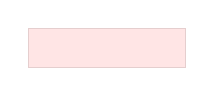
\begin{tikzpicture}
\draw[fill=red,opacity=0.1](0,0) rectangle (2,0.5);
\end{tikzpicture}
\end{textblock*}
\end{frame}

\begin{frame}{Single Task Flexibility (Task View)}
\includegraphics[width=11cm]{images/mt10taskfreedom}
\begin{textblock*}{4.5cm}(11cm,3cm)
\begin{itemize}
\item Bounds best viewed in task view
    \item Difficult to make fully interactive 
    \item Extra constraints can be a challenge
\end{itemize}
\end{textblock*}
\end{frame}


\section{Summary}

\begin{frame}{What have we discussed?}
\begin{itemize}
    \item How to use visualization in modelling problems
    \item How this integrates into development process
    \item What can be done with different tools
    \item Overview of literature in this area
\end{itemize}    
\end{frame}

\begin{frame}{What did we leave out?}
\only<1>{\begin{textblock*}{6cm}(8cm,0cm)
\includegraphics[width=6cm]{images/explainingalldifferent.PNG}

{\scriptsize from \cite{DBLP:conf/acsc/DowningFS12}}
\end{textblock*}}

\only<2>{\begin{textblock*}{6cm}(8cm,0cm)
\includegraphics[width=6cm]{images/graphcoloring}
\end{textblock*}}

\only<3>{\begin{textblock*}{6cm}(8cm,0cm)
\includegraphics[width=6cm]{images/dooms}
\end{textblock*}}

\only<4>{\begin{textblock*}{6cm}(8.5cm,0cm)
\includegraphics[width=6cm]{images/visualizationevaluation.PNG}
\tiny from: \cite{DBLP:journals/tvcg/SaketED19}
\end{textblock*}}

\only<5>{\begin{textblock*}{6cm}(8.5cm,0cm)
\includegraphics[width=6cm]{images/moses.pdf}
\tiny from: COSYTEC. Moses Feedmill Scheduling System
\end{textblock*}}

\only<6>{\begin{textblock*}{4.5cm}(8.5cm,0cm)
\includegraphics[width=4.5cm]{images/A-domino-portrait-of-George-Boole-generated-by-our-approach-using-49-sets-of-double.png}
\end{textblock*}}

\only<7>{\begin{textblock*}{5cm}(8cm,0cm)
\includegraphics[width=7cm]{images/ganttscalability.PNG}
\end{textblock*}}

\begin{itemize}
    \item<+-|alert@+> Visualizations to understand and\\ improve a solver
    \item<+-|alert@+> Tools for Constraint Acquisition
    \item<+-|alert@+> Visualization for Local Search and\\ Constraint Based Local Search\\\cite{DBLP:journals/constraints/DoomsHM09}
    \item<+-|alert@+> How to test effectiveness of visualization
    \item<+-|alert@+> Visualizations for specific applications
    \item<+-|alert@+> Visualization as opt-art\\ \cite{DBLP:conf/cpaior/Bosch06,DBLP:journals/anor/CambazardHOO11}
    \item<+-|alert@+> Scalability issues
\end{itemize}    
\end{frame}

\begin{frame}{Are the Examples Available?}
\begin{itemize}
    \item Much is available in the MiniZinc IDE
    \item Assistant based material not yet released
    \item Will become available as open-source
    \item Slide set available at \url{}
\end{itemize}    
\end{frame}


\section{Bibliography}


\nocite{DBLP:conf/discipl/SimonisCDFNT00}
\nocite{DBLP:journals/tvcg/LiuDTGM21}
\nocite{DBLP:journals/tvcg/GoodwinMDBTW17}
\nocite{DBLP:journals/constraints/ShishmarevMTB16}
\nocite{DBLP:conf/ppdp/CameronBMM03}
\nocite{DBLP:conf/cp/Meier95}
\nocite{DBLP:conf/discipl/CarroH00}
\nocite{DBLP:conf/discipl/CarroH00a}
\nocite{DBLP:conf/agp/CarroH98}
\nocite{DBLP:conf/discipl/DeransartHM00}
\nocite{DBLP:conf/iclp/Deransart04}
\nocite{DBLP:journals/constraints/DoomsHM09}
\nocite{DBLP:conf/cpaior/LeoT17}
\nocite{DBLP:journals/constraints/FagesSC04}
\nocite{DBLP:conf/softvis/GhoniemCFJ05}

\begin{frame}[allowframebreaks]
\frametitle{References}
\bibliographystyle{apalike}
\bibliography{bib}
\end{frame}

